% fontes.tex %%%%%%%%%%%%%%
\begin{frame}[standout]
  \huge
  \filename{fontes.tex}
\end{frame}

% MetaFont era o sistema original, mas hoje usamos principalmente fontes do
% tipo OpenType
\begin{frame}
  \frametitle{\filename{fontes.tex}}
  \Huge
  \MF, Truetype (\code{ttf}) \& OpenType (\code{otf})
\end{frame}

% Na tabela ASCII, há apenas 95 caracteres imprimíveis. Nenhum deles é
% acentuado.
\begin{frame}[plain]
  \hspace*{-11.5mm}
  \begin{centering}
    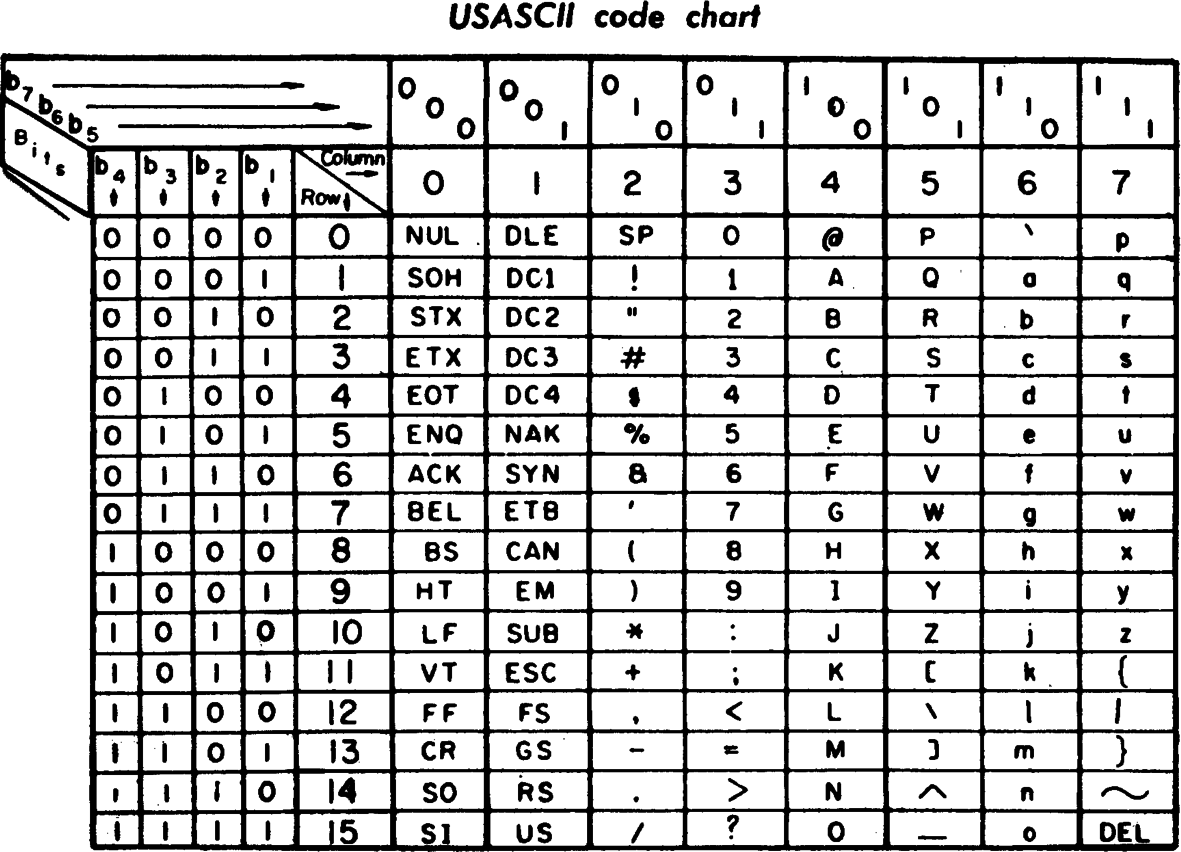
\includegraphics[width=\paperwidth]{imagens/ascii-chart}
    \par
  \end{centering}
\end{frame}

% A primeira codificação ficou conhecida como OT1 e a maior parte dos
% caracteres veio da tabela ASCII. Sintaxe para inserir acentos.
\begin{frame}[fragile]
  \frametitle{\filename{fontes.tex}}
  \huge
  \code{OT1}: Old Text 1
  \vspace{1em}

  \verb+Eur\'{i}pides+: Eur\'{i}pides
\end{frame}

% Hoje não temos que nos preocupar com codificação, inserção de acentos etc.
\begin{frame}
  \frametitle{\filename{fontes.tex}}
  \Huge
  Hoje em \LaTeX, temos a codificação de fonte \code{TU}
\end{frame}

% O pacote fontspec é carregado automaticamente pelo polyglossia, mas
% carregaremos ele mesmo assim.
\begin{frame}[fragile]
  \frametitle{\filename{fontes.tex}}
  \huge
  Aproveitar as vantagens do Unicode:

  \begin{minted}[autogobble,fontsize=\huge,breaklines]{latex}
    \usepackage{fontspec}
  \end{minted}
\end{frame}

% Exemplo do que podemos fazer usando LaTeX e Unicode. É claro, a fonte tem que
% conter os caracteres que estamos tentando usar.
\begin{frame}
  \frametitle{\filename{fontes.tex}}
  \Huge
  Εὐριπίδης — meu amigo de tantos anos — só lê Достое́вский.
\end{frame}

% Vamos aprender a acessar os diversos tipos de uma família de fontes. Vamos
% discutir com mais profundidade no exemplo e exercício.
\begin{frame}[fragile]
  \frametitle{\filename{fontes.tex}}
  \Huge
  \only<1>{Fontes vêm em famílias}
  \only<2>{\mintinline{latex}{\textrm}: \textrm{romanas}}
  \only<3>{\mintinline{latex}{\emph}: \emph{ênfase}}
  \only<4>{\mintinline{latex}{\textbf}: \textbf{negrito}}
  \only<5>{\mintinline{latex}{\textsc}: \textsc{Versaletes}}
  \only<6>{\mintinline{latex}{\texttt}: \texttt{teletipo}}
\end{frame}

% Tamanhos de fontes em LaTeX. Geralmente não é uma boa ideia usar eles à mão,
% pois os designers das classes de documento tomam essas decisões para nós.
\begin{frame}[fragile]
  \frametitle{\filename{fontes.tex}}
  \large
  Tamanhos de fonte:
  \begin{multicols}{2}
    \begin{itemize}
      \item{\code{\textbackslash tiny}: 5pt}
      \item{\code{\textbackslash scriptsize}: 7pt}
      \item{\code{\textbackslash footnotesize}: 8pt}
      \item{\code{\textbackslash small}: 9pt}
      \item{\code{\textbackslash normalsize}: 10pt}
      \item{\code{\textbackslash large}: 12pt}
      \item{\code{\textbackslash Large}: 14pt}
      \item{\code{\textbackslash LARGE}: 17pt}
      \item{\code{\textbackslash huge}: 20pt}
      \item{\code{\textbackslash Huge}: 25pt}
    \end{itemize}
  \end{multicols}
\end{frame}

\begin{frame}
  \frametitle{\filename{fontes.tex}}
  \begin{quote}
    \underline{\textbf{Remember\Huge!}} \textit{The}
    \textsf{M\textbf{\LARGE O} \texttt{R}\textsl{E}} fonts \Huge you
    \tiny use \footnotesize \textbf{in} a \small \texttt{document},
    \large \textit{the} \normalsize more \textsc{readable} and
    \textsl{\textsf{beautiful} it bec\large o\Large m\LARGE e\huge s}.
  \end{quote}
\end{frame}

% Como trocar as fontes. Explicar que fontes matemáticas são outra história.
\begin{frame}[fragile]
  \frametitle{\filename{fontes.tex}}
  \Large
  Carregar fontes usando o \code{fontspec}:

  \begin{minted}[autogobble,fontsize=\Large,breaklines]{latex}
    \usepackage{fontspec}
      \setmainfont{Linux Libertine}
  \end{minted}
\end{frame}

% Fontes devem estar nos diretórios padrão. Caso não estejam, podemos
  % especificar um diret´orio:
\begin{frame}[fragile]
  \frametitle{\filename{fontes.tex}}
  \Large
  Especificar um diretório:

  \begin{minted}[autogobble,fontsize=\Large,breaklines]{latex}
    \usepackage{fontspec}
      \setmainfont{Linux Libertine}[
        Path = fonts/
      ]
  \end{minted}
\end{frame}

% Ligaduras são sequências de letras que naturalmente colidem. Por isso, são
% substituídas por outro caractere.
\begin{frame}
  \frametitle{\filename{fontes.tex}}
  \Huge
  Linux Libertine e ligaduras

  \fontspec{Linux Libertine}{
    affair\qquad fjord\qquad flor\\
    af\mbox{}fair\qquad f\mbox{}jord\qquad f\mbox{}lor
  }
\end{frame}

% Antes do exercício, vamos rever os conceitos que discutimos de maneira
% prática.
\begin{frame}
  \frametitle{\filename{fontes.tex}}
  \Huge
  Demonstrar ideias em \filename{fontes.tex}
\end{frame}

% Resolver o exercício fontes-exercicio.tex.
\begin{frame}
  \frametitle{\filename{fontes.tex}}
  \Huge
  Resolver \filename{fontes-exercicio.tex}
\end{frame}
